\section{Wstęp}
Porównuję dokładność sieci rodzaju MLP w zależności od ilości danych - 
podczas uczenia sieci wycinkiem danych uczących, dokładność sieci wzrasta do granicznej 88,34\% przy wykorzystaniu pełnego zestawy danych uczących.
Zmiana ilości neuronów w dwu warstwach również wpływa na dokładność sieci i jest największa przy 64 neuronach. Zwiększenie lub zmniejszenie liczby neuronów zmniejsza dokładność sieci. Długość procesu uczenia wynosiła 5000 epok. Szacowanie przeprowadzałem w języku Matlab. Metodę uczenia wybrałem metodę największego spadku, ponieważ przy wyborze metody LM miałem za mało pamięci dla takiej konfiguracji sieci. (wymagane 21Gb)


\begin{figure}[h]
    \begin{subfigure}{.5\textwidth}
    	\centering 
            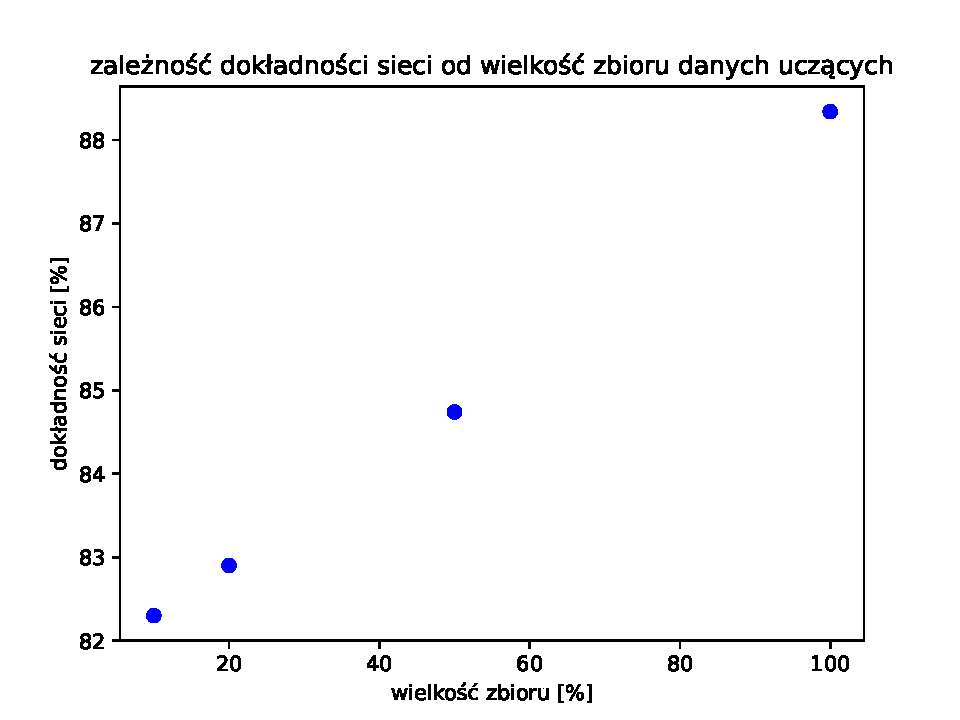
\includegraphics[width=0.90\linewidth]{gfx/fig03b.pdf} 
    \end{subfigure} %
    \begin{subfigure} {.5\textwidth}
    	\centering 
            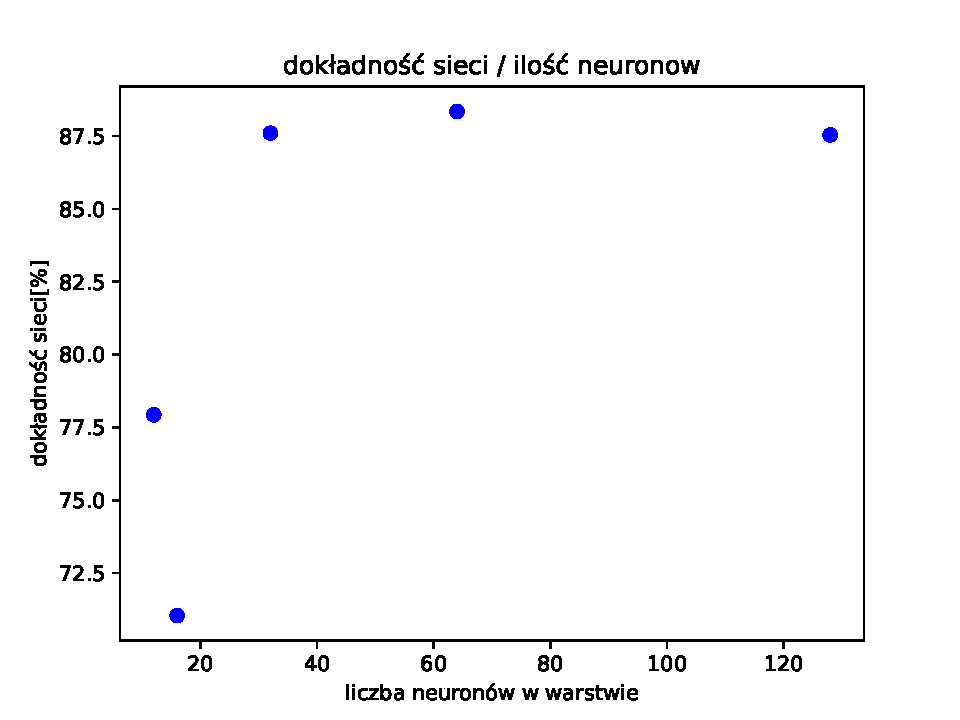
\includegraphics[width=0.90\linewidth]{gfx/fig03a.pdf} 
    \end{subfigure} 
    \caption{Szacowanie parametrów sieci}
\end{figure} 

Porównanie czasów wykonania uczenia 64 neuronów w 2 warstwach i 5000 epok dla różnych języków. 
Dla Matlab wyniki uzyskane w systemie operacyjnym Windows 10 oraz Arch Linux w trybie tekstowym, dodatkowo wyniki przy obliczeniach domyślnych proponowanych przez program, w porównaniu z wymuszeniem obliczeń tylko na GPU. Dość zaskakująca jest różnica w szybkości obliczeń na GPU w zależności od platformy. Odpowiednio w systemie Windows 10 obliczenia trwają 419-425 sek., Linux Arch wykona te obliczenia w czasie 205-211 sek. 
\section{Dane treningowe}
Dane treningowe i testowe - zestaw pisanych ręcznie cyfr - pochodzą z zasobów MNIST (yann.lecun.com). w kodzie Java dodałem zestaw metod umożliwiający m.in. podejrzenie wektorów treningowych jako obrazy, zapisanie wag warstwy jako obraz, i inne.

\begin{figure}[h]
	\centering 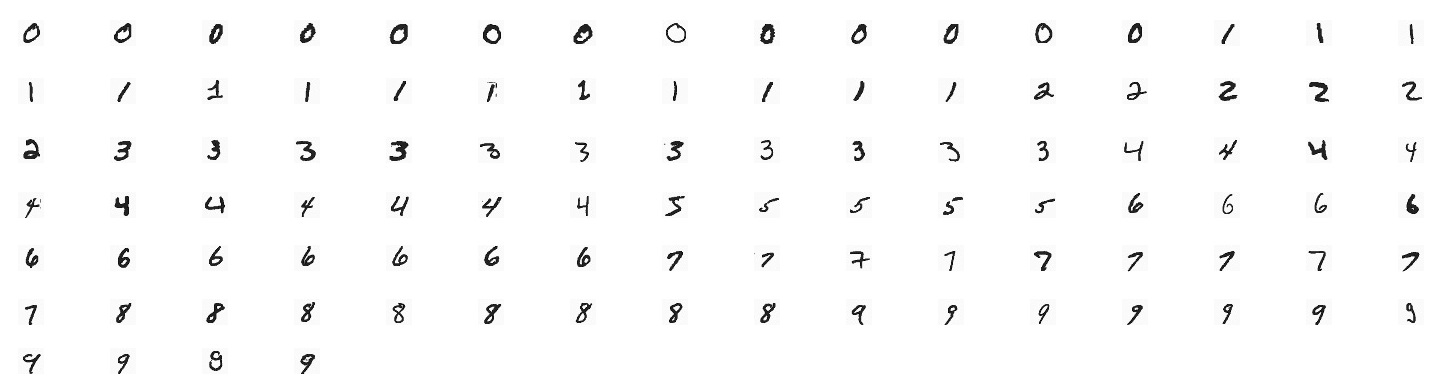
\includegraphics[width=0.9\textwidth]{gfx/mnist_prev.png} 
	\caption{ podgląd próbki wektorów uczących}
	\label{rys:podglad_mnist}
\end{figure}

poniżej kod ładujący dane, oraz metody narzędziowe:

\begin{lstlisting}[ basicstyle=\tiny]

public  void prepareData( int percent ){
   trainYfile =  loadBin( "../data/" + "t10k-images-idx3-ubyte", 8, percent*600 ); //offset=8, size=percent*600  // OK
   testYfile =  loadBin( "../data/" + "t10k-labels-idx1-ubyte",  8, percent*100 ); // offset=8, size=percent*100 // OK

   trainY = new float[percent*600][];
   testY  = new float[percent*100][];
   //train Y
   for (int i=0;i<percent*600;i++){
      trainY[i] = new float[]{ 0.0f, 0.0f, 0.0f, 0.0f, 0.0f, 0.0f, 0.0f, 0.0f, 0.0f, 0.0f };
      trainY[i][ trainYfile[i] ]=1.0f;
   }

   byte[] trainXfile = loadBin(path + trainXname, 16, percent * 784 * 600);// offset=16 size=percent*784*600
      trainX=new float[percent*600][784];
         for (int i=0;i<percent*100;i++) {
            int off=i*784;
            for (int j=0;j<784;j++){
               trainX[i][j]=Byte.toUnsignedInt( trainXfile[off+j] )/16; 
               
        }}} catch (IOException e) { throw new RuntimeException(e); }
   }


    public static byte[] loadBin( String filename, int offset, int len ) throws IOException {
        byte[] bytesBuf = new byte[ len ];
        File f = new File( filename );
        FileInputStream fis = new FileInputStream( filename );
        fis.skip(offset);
        fis.read( bytesBuf, 0, len );
        return bytesBuf;
    }

    public static float[] vectorSubstSsubZ( float[] s, float[] z ){
        float[] out = new float[ z.length];
        for ( int i=0;i<z.length; i++ ){
            out[i] = ( s[i] - z[i] );
        }
        return out;
    }

    public static float meanSquareError( float[] s, float[]z ){
        float out = 0.0f;
        for ( int i=0;i<z.length; i++ ){
            float delta = s[i] - z[i];
            out+=delta*delta;
        }
        return out;
    }
 
    public static BufferedImage arrayOfFloatToImage( float[] data , int xScale ){
        int width = data.length/xScale;
        int height = 510;
        float min = data[0];
        float max = data[0];
        for ( int i=1;i< data.length;i++ ){
            if ( data[i]<min ) { min=data[i]; }
            if ( data[i]>max ) { max=data[i]; }
        }
        float delta=( max-min )/(height-10);
        BufferedImage image = new BufferedImage( width , height , TYPE_INT_RGB );

        int pointColor = (255*255*240)+(255*244)+244;
        for ( int i=0;i<width;i++ ){
            int val=(int) (( data[xScale*i]-min )/delta ) ;
            image.setRGB( i, 5+val , pointColor );
        }
        return image;
    }

    public static void saveImg( BufferedImage image, String nameSuffix ){
        File file = new File("image"+nameSuffix+".png");
        try {
            ImageIO.write(image ,  "png", file );
        } catch (IOException e) {
            throw new RuntimeException(e);
        }
    }
}
\end{lstlisting}

\section{Uzyskane wyniki}
\begin{figure}[h]
    	\centering 
            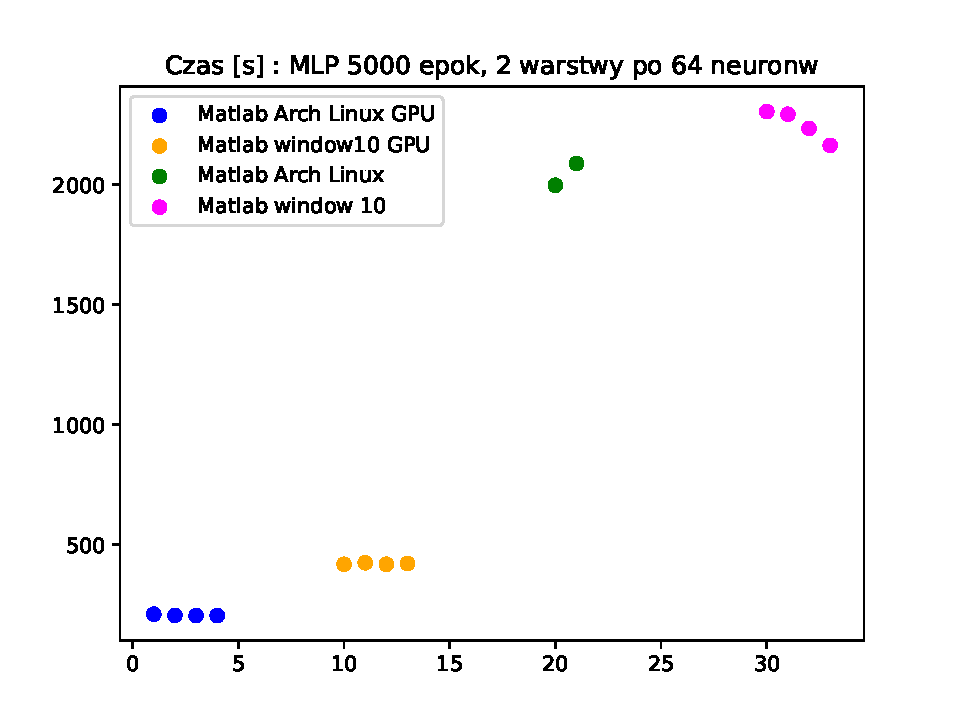
\includegraphics[width=0.88\linewidth]{gfx/fig03.pdf} 
\end{figure} 


\newpage
\section{Kod realizujący obliczenia}

Matlab:
\begin{lstlisting}

    net = feedforwardnet([ 64, 64 ],'traingd'); 
    net.trainParam.epochs = 5000;
    net.trainParam.goal   = 0.03;
    net.input.processFcns = {'mapminmax'};  

    gxtrain = gpuArray( xtrain );
    gytrain = gpuArray( ytrain );

    ST = datetime('now');

    gpu=true;
    if ( gpu )
        %GPU
        net = configure(net,xtrain,ytrain);
        net = train(net, gxtrain, gytrain,'useParallel','yes','useGPU','yes');
    else
        %No GPU
        net = train( net, xtrain, ytrain );
    end    
    
    ED = datetime('now');

    z = net( xtest );
    flatZ = aryOfVectorToAryOfInt( z );
    flatZtest = aryOfVectorToAryOfInt( ytest ); 
    accuracy = accuracyCheck(flatZ, flatZtest);

    D = duration( ED-ST );

    fprintf('# MLP: 2x64Neu * 5000 cycles:\n' );
    fprintf( '# accuracy: a:%f\n\n' , accuracy );
    fprintf ('m[]=%f\n' , seconds(D)  );

\end{lstlisting}

\newpage
\section{Własna implementacja w Java}
Do napisania programu użyłem własnego, opisanego we wcześniejszych rozdziałach modelu obiektowego sieci neuronowych. Sieć ta pracuje dużo wolniej niż rozwiązanie w matlab, uczenie sieci zajmuje aż 14400 sek. Najważniejszym celem napisania tego programu było sprawdzenie czy sieć oparta na modelu obiektowym działa, i czy osiągnie podobny poziom dokładności jak gotowe rozwiązanie z Matlab. Okazuje się, że podobnie jak sieć w Matlab, ta napisana w Java osiąga dokładność około 87\%;
Kod celowo nie jest optymalizowany pod kątem wydajności  - chodziło mi o łatwość czytania i zrozumienia modelu, a także potwierdzenie że sieć oparta na tym modelu uczy się podobnie jak gotowe rozwiązanie z Matlab. W kodzie umieściłem metody dzięki którym mogłem sprawdzić czy dane wczytują się prawidłowo. Poniżej zamieszczam kod rozwiązania:
\begin{lstlisting} [ basicstyle=\tiny]
// main.java
private float[][] testX; private float[][] testY; private float[][] trainX; private float[][] trainY;

private Layer layer1; private Layer layer2; private Layer layer3;

private Tools tools = new Tools();
int numOfEpoch=500;
float[] CSBin_data=new float[numOfEpoch];

public void prepare() {
    tools.prepareData( 100 );
    testX = tools.getTestX();
    testY = tools.getTestY();
    trainX = tools.getTrainX();
    trainY = tools.getTrainY();

    layer1=new Layer( LType.sigmod , 64 ,784 ); layer1.setName("Layer1"); // n neurons
    layer2=new Layer( LType.sigmod , 64 ,64 ); layer2.setName("Layer2"); // n neurons
    layer3=new Layer( LType.softmaxMultiClass , 10 ,64 ); layer3.setName("Layer3"); // n neurons
    layer1.rnd();  layer2.rnd();  layer3.rnd();
}

public void run() {

float Loss = 0.0f;
for (int epoch = 0; epoch < numOfEpoch; epoch++) {
    for ( int index = 0; index < trainX.length; index++ ) {
        layer1.setX( trainX[ index ] );
        layer1.nForward();
        layer2.setX( layer1.getZ() );
        layer2.nForward();
        layer3.setX( layer2.getZ() );
        layer3.nForward();

        float[] S_Z = tools.vectorSubstSsubZ( trainY[ ind_ex ], layer3.getZ() );
        layer3.nBackward( S_Z );
        layer2.nBackward( layer3.getEout() );
        layer1.nBackward( layer2.getEout() );
    }
}
        // check accuracy
int len = testX.length;
int accuracy = 0;
for (int i = 0; i < len; i++) {
    layer1.setX( testX[i] );
    layer1.nForward();
    layer2.setX( layer1.getZ() );
    layer2.nForward();
    layer3.setX( layer2.getZ() );
    layer3.nForward();

    int netClassId = tools.getIndexMaxFloat( layer3.getZ() );
    int fileClassId = tools.getIndexMaxFloat( testY[i] );
    if (fileClassId == netClassId) { accuracy++; }
    }
System.out.println(100.0f * accuracy / len + "%");
}}\end{lstlisting}

\begin{lstlisting} [ basicstyle=\tiny]
// neuron.java
public class Layer {
    private String name;
    private  LType lType;
    private  Neuron[] neurons;
    private  float X[];
    private  float Y[];
    private  float Z[];
    private  float dFofZ[];
    private  float Eout[]; // S-Z for last

    public Layer( LType lType, int n, int m ) {// n - number of neurons & output size Y[n], Z[n]
        this.lType=lType;                      // m - number of inputs  = input  size X[m]
        this.neurons = new Neuron[n];
        for (int i=0; i<n; i++){
            this.neurons[i]=new Neuron(m, this);
        }
        X = new float[m];
        Y = new float[n];
        Z = new float[n];
        dFofZ = new float[n];
        Eout = new float[m];
    }

    public void setWmn( int n, int m, float wji ){ neurons[n].setWm( m, wji ); }

    public void rnd(){
        Random random=new Random();
        for ( Neuron neu : neurons ) {
            for ( int m=0; m<X.length; m++ ) {
                neu.setWm( m , (float)( -1.0f+2.0f*random.nextFloat() )  );
            }
        }
    }

    public float[] nForward() {
        switch (lType) {
            case sigmod:
            case sigmod_CrossEntropy_Binary:{
                for (int n = 0; n < neurons.length; n++) {
                    Y[n] = neurons[n].Forward(X);
                    Z[n] = F(Y[n]);
                    dFofZ[n] = dF(Z[n]);
                }
                for (int m=0;m<Eout.length;m++){ Eout[m]=0; }
                return Z;
            }
            case softmaxMultiClass: {
                int len = neurons.length;
                float sum = 0.0f;
                float max = Y[0] = neurons[0].Forward(X);
                for (int i=1;i<len;i++){
                    dFofZ[i] = 1;
                    Y[i]=neurons[i].Forward(X);
                    if (Y[i]>max) { max=Y[i]; }
                }
                for (int i = 0; i < len; i++) {
                    Y[i] = (float) Math.exp( Y[i]-max );
                    sum += Y[i];
                }
                for (int i = 0; i < len; i++) {
                    Z[i] = Y[i] / sum;
                }
                return Z;
            }
            default: { return Z; }
        }
    }

    public void nBackward( float[] Ein ){ // S-Z or Ein
        for ( int i=0;i<neurons.length;i++ ){ Eout[i]=0.0f; }
        for ( int n=0; n< neurons.length; n++ ){
            neurons[n].Backward( Ein[n] * dFofZ[n] );
        }
    }




    private float F ( float y ){
        float z;
        switch (this.lType) {
            case sigmod:
            case sigmod_CrossEntropy_Binary:
                { z = (float) (1.0f/(1.0f + Math.exp( -y ))); break; }
            case linear:
                default: { z=y; break; }
        }
        return z;
    }

    private float dF ( float z ){
        float df;
        switch (lType) {
            case sigmod:
                { df = z*(1-z); break; }
            case linear:
            case sigmod_CrossEntropy_Binary:
            default: { df=1; break; }
        }
        return df;
    }

    // getters / setters
    public void setX( float[] _x ) {
        for ( int m=0; m<X.length; m++ ){
            this.X[m] = _x[m];
        }
    }
    public float[] getZ() { return Z; }
    public float[] getX() { return X; }
    public float[] getEout() { return Eout; }
}\end{lstlisting}

\begin{lstlisting} [ basicstyle=\tiny]
// neuron.java
public class Neuron {
    private float bias=0;
    private final float[] W;
    private final Layer parent;
    private final static float mu=0.001f;

    public void setBias( float b ) { this.bias=b; }
    public float getBias(){ return bias; }

    public Neuron( int m, Layer parent ) {
        this.parent=parent;
        this.W = new float[m];
    }

    public void setWm( int m, float wji ){
        W[m] = wji; 
    }

    public float Forward( float[] X ) {
        float res=bias;
        for ( int m=0; m<W.length; m++ ) {
            res+= X[m]*W[m];
        }
        return res;
    }

    public void Backward( float en_x_dFIznI ) {
        float[] X = parent.getX();
        for ( int m=0; m<W.length; m++ ) {
            parent.getEout()[m] += ( W[m] * en_x_dFIznI );
            W[m] += mu * en_x_dFIznI * X[m];
        }
    }
}
\end{lstlisting}

\section{Pyton}
Python -numpy, -sklearn
\begin{lstlisting}
   ?
\end{lstlisting}

c) Python -tensorflow
\begin{lstlisting}
   ?
\end{lstlisting}








